%! TEX root = ../../master.tex
\lecture[Representation of polyhedra. Theorem of the Alternative and applications. Non-linearity in LP.]{Do 05 May 2022}{Theorem of the Alternative}
\begin{theorem}[Minkowski] \label{thm:minkowski}
    For a polyhedron $P$ it holds $x \in P$ iff there exist vertices $v_1,...,v_k$
    and rays $r_1, ..., r_l$, such that
    \begin{align*}
        \sum_i \lambda v_i + \sum_j \mu_j r_j & = x     \\
        \sum_i \lambda_i                      & = 1     \\
        \lambda, \mu                          & \geq 0.
    \end{align*}
    \vocab{Minkowski's Theorem} is also known as \vocab{Resolution Theorem}.
\end{theorem}
\begin{proof}
    See ADM1.
\end{proof}
\begin{definition}
    We have different variants of representing a polyhedron $P$:
    \begin{itemize}
        \item The \vocab[polyhedron!H-representation]{H-representation} (from "hyperplane") is given by $P=\{x \mid Ax \leq b\}$.
        \item The \vocab[polyhedron!V-representation]{V-representation} (from "vertex") is given by \autoref{thm:minkowski}.
    \end{itemize}
\end{definition}
\begin{conclusion}
    Depending on the representation we have, we have different ways to solve $\OPT$ and $\SEP$:
    \\
    \begin{center}
        \begin{tabular}{rll}
                                        & H-representation                          & V-representation                           \\ \cline{2-3}
            \multicolumn{1}{r|}{$\OPT$} & \multicolumn{1}{l|}{LP Simplex/Ellipsoid} & \multicolumn{1}{l|}{Brute Force}           \\ \cline{2-3}
            \multicolumn{1}{r|}{$\SEP$} & \multicolumn{1}{l|}{Brute Force}          & \multicolumn{1}{l|}{LP (\autoref{ex:4.1})} \\ \cline{2-3}
        \end{tabular}
    \end{center}

\end{conclusion}
\begin{example}
    Consider the $n$-cube $C^n \coloneqq \{x \in \realnum^n \mid -1 \leq x_i \leq 1\}$.
    It has $2n$ facets, but $2^n$ vertices.

    Now, consider the polar of $C^n$, which can be shown to be the $n$-octahedron $O^n$.
    Remember the intuition, that the polar exchanges vertices with facets. Indeed it holds that
    now, we have $2^n$ facets, but only $2n$ vertices.

    \begin{minipage}{\textwidth}
        \centering
        \begin{minipage}{0.4\textwidth}
            \centering
            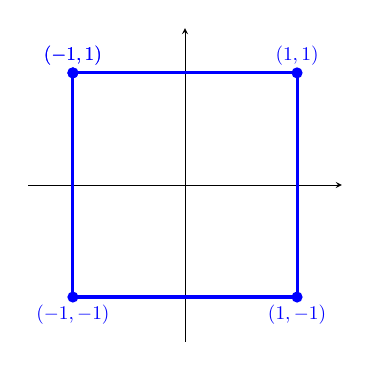
\begin{tikzpicture}[scale=0.7]
                \begin{axis}[
                        axis y line=center,
                        axis x line=middle,
                        xmin=-1.4,
                        xmax=1.4,
                        ymin=-1.4,
                        ymax=1.4,
                        grid=none,
                        ticks=none,
                        % minor tick num=1,
                        axis equal image,
                        nodes near coords={
                                $(\pgfmathprintnumber{\pgfkeysvalueof{/data point/x}},
                                    \pgfmathprintnumber{\pgfkeysvalueof{/data point/y}})$
                            },
                    ]
                    \addplot[mark=*,blue, ultra thick] coordinates {(-1,1) (1,1) (1,-1) (-1,-1) (-1,1)};
                \end{axis}
            \end{tikzpicture}
        \end{minipage} $\overset{\text{polar}}{\longleftrightarrow}$
        \begin{minipage}{0.4\textwidth}
            \centering
            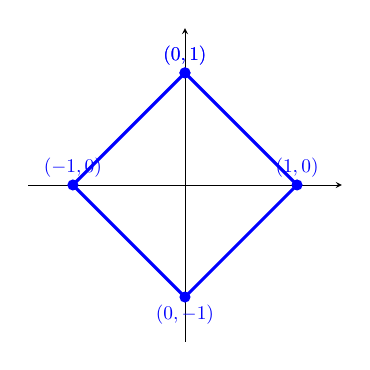
\begin{tikzpicture}[scale=0.7]
                \begin{axis}[
                        axis y line=center,
                        axis x line=middle,
                        xmin=-1.4,
                        xmax=1.4,
                        ymin=-1.4,
                        ymax=1.4,
                        grid=none,
                        ticks=none,
                        % minor tick num=1,
                        axis equal image,
                        nodes near coords={
                                $(\pgfmathprintnumber{\pgfkeysvalueof{/data point/x}},
                                    \pgfmathprintnumber{\pgfkeysvalueof{/data point/y}})$
                            },
                    ]
                    \addplot[mark=*,blue, ultra thick] coordinates {(0,1) (1,0) (0,-1) (-1,0) (0,1)};
                \end{axis}
            \end{tikzpicture}
        \end{minipage}
        \captionof{figure}{2-cube vs. 2-octahedron}
    \end{minipage}

    \begin{minipage}{\textwidth}
        \centering
        \begin{minipage}{0.4\textwidth}
            \centering
            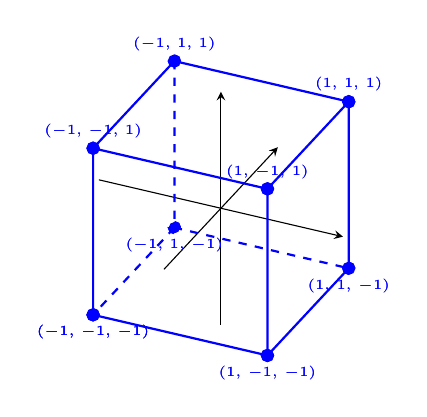
\begin{tikzpicture}
                \begin{axis}[
                        axis y line=center,
                        axis x line=middle,
                        axis z line=middle,
                        xmin=-1.4,
                        xmax=+1.4,
                        ymin=-1.4,
                        ymax=+1.4,
                        zmin=-1.4,
                        zmax=+1.4,
                        scale=1.3,
                        ticks=none,
                        axis equal image,
                        nodes near coords style={font=\tiny},
                        nodes near coords={
                                (\pgfmathprintnumber{\pgfkeysvalueof{/data point/x}},
                                \pgfmathprintnumber{\pgfkeysvalueof{/data point/y}},
                                \pgfmathprintnumber{\pgfkeysvalueof{/data point/z}})
                            },
                    ]
                    \addplot3[mark=*,blue, thick, dashed] coordinates {(-1,1, 1) (-1,1, -1) (1,1,-1)};
                    \addplot3[mark=*,blue, thick, dashed] coordinates {(-1,1, -1) (-1,-1, -1)};
                    \addplot3[mark=*,blue, thick] coordinates {(-1,-1,-1) (-1,-1,1) (-1,1,1) (1,1,1) (1,1,-1) (1,-1,-1) (-1,-1,-1)};
                    \addplot3[mark=*,blue, thick] coordinates {(1,-1,-1) (1,-1,1) (-1,-1,1)};
                    \addplot3[mark=*,blue, thick] coordinates {(1,-1,1) (1,1,1)};
                \end{axis}
            \end{tikzpicture}
        \end{minipage} $\overset{\text{polar}}{\longleftrightarrow}$
        \begin{minipage}{0.4\textwidth}
            \centering
            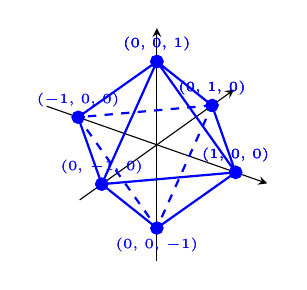
\begin{tikzpicture}
                \begin{axis}[
                        axis y line=center,
                        axis x line=middle,
                        axis z line=middle,
                        % xrotate=20,
                        view={35}{30},
                        xmin=-1.4,
                        xmax=+1.4,
                        ymin=-1.4,
                        ymax=+1.4,
                        zmin=-1.4,
                        zmax=+1.4,
                        scale=1.3,
                        ticks=none,
                        axis equal image,
                        nodes near coords style={font=\tiny},
                        nodes near coords={
                                (\pgfmathprintnumber{\pgfkeysvalueof{/data point/x}},
                                \pgfmathprintnumber{\pgfkeysvalueof{/data point/y}},
                                \pgfmathprintnumber{\pgfkeysvalueof{/data point/z}})
                            },
                    ]
                    \addplot3[mark=*,blue, thick, dashed] coordinates {(0,1,0) (-1,0,0) (0,0,-1) (0,1,0)};
                    \addplot3[mark=*,blue, thick] coordinates {(0,0,1) (0,-1,0) (1,0,0) (0,0,1) (0,1,0) (1,0,0)};
                    \addplot3[mark=*,blue, thick] coordinates {(1,0,0) (0,0,-1) (0,-1,0) (-1,0,0) (0,0,1)};
                \end{axis}
            \end{tikzpicture}
        \end{minipage}
        \captionof{figure}{3-cube vs. 3-octahedron}
    \end{minipage}

\end{example}
\begin{info}
    \href{https://polymake.org/doku.php}{Polymake} is a tool for converting programmatically between H\-/representation and V\-/representation.
\end{info}
\subsection{Certificate construction}
\begin{question}
    Consider the problem of finding a solution $x$ to a linear or integer system.
    How do we construct succinct certificates of feasibility and infeasibility?
\end{question}
In order to answer this question, we will have to look at different kinds of systems each on their own.
For the following theorems, we will consider two different systems every time, and show that the solutions
can be used as the certificate we seek for.
\begin{theorem}
    Exactly one of the following systems is feasible:
    \begin{align*}
        Ax & =b & \text{vs.} &  & y^TA & =0 \\
           &    &            &  & y^Tb & =1
    \end{align*}
    In particular, the left system delivers a certificate of feasibility, whereas the right a certificate of infeasibility.
\end{theorem}
\begin{proof}
    Suppose both are feasible. Then we have solutions $y^0,x^0$, and can construct following contradiction:
    \begin{alignat*}{2}
                              &  & Ax^0                        & = b            \\
        \Leftrightarrow \quad &  & \underbrace{(y^0)^TA}_0 x^0 & = (y^0)^Tb = 1
    \end{alignat*}
    It remains to prove at least one system is feasible. We can use \vocab{Gaussian Elimination} for that:
    Gaussian Elimination either yields a solution $x^0$ we can use as a succinct certificate for feasibility,
    or determine it is infeasible by yielding the row multiplier $y^0$ in order to generate $0^Tx=1$ as a succinct certificate of infeasibility.
\end{proof}
\begin{warning}
    Gaussian Elimination is \emph{not} polynomial in its natural variant because of numbers generated during the algorithm.
    Nonetheless, if careful and using certain tricks, Gaussian Elimination is polynomial.
\end{warning}
\begin{remark}
    Theorems stating that exactly one of two systems have a solution are called \vocab{Theorem of the Alternative}.
\end{remark}
\begin{theorem}[\vocab{Farkas' Lemma}]
    \label{thm:farkas}
    Exactly one of the following systems is feasible:
    \begin{align*}
        Ax & \leq b & \text{vs.} &  & y^TA & =0     \\
           &        &            &  & y^Tb & <0     \\
           &        &            &  & y    & \geq 0 \\
    \end{align*}
    In particular, the left system delivers a certificate of feasibility, whereas the right a certificate of infeasibility.
\end{theorem}
\begin{proof}
    Suppose both are feasible. Analoguous to previous proof we can see the contradiction:
    \begin{alignat*}{2}
                              &  & Ax^0                        & \leq b            \\
        \Leftrightarrow \quad &  & \underbrace{(y^0)^TA}_0 x^0 & \leq (y^0)^Tb < 0
    \end{alignat*}
    At least one system is feasible, which we can see by using the Ellipsoid Method to get a feasible $x$ as a feasibility certificate for $Ax \leq b$. Otherwise, $Ax\leq b$ is infeasible.
    In that case we can use Phase 1 of the Simplex Method to generate $0^Tx \leq z$ (for some $z \in \integers^-$) and use the extracted row multipliers $y$ as an infeasibility certificate.
    Note that this $y$ solves the right system.
\end{proof}
\begin{conclusion}
    We already knew from \autoref{thm:LP-NP} and \autoref{thm:LP-coNP}, that previous feasibility problems both lie in $\NP \cap \coNP$.
    Thus, we found that Gaussian Elimination is the suspected polynomial algorithm.
\end{conclusion}
\begin{definition}[Diophantine equations]
    An equation of the form $Ax=b$, for $x \in \integers^n$, is called \vocab{diophantine equation}.
\end{definition}
\begin{theorem}
    Exactly one of following systems is feasible:
    \begin{align*}
        Ax & = b             & \text{vs.} &  & y^TA & \in \integers^n    \\
        x  & \in \integers^n &            &  & y^Tb & \not \in \integers \\
    \end{align*}
    In particular, the left system delivers a certificate of feasibility, whereas the right a certificate of infeasibility.
\end{theorem}
\begin{proof}
    Suppose both are feasible. Then
    \begin{alignat*}{2}
                              &  & Ax^0                                                               & = b                                          \\
        \Leftrightarrow \quad &  & \underbrace{(y^0)^TA}_{\integers^n} \underbrace{x^0}_{\integers^n} & = \underbrace{(y^0)^Tb}_{\not \in \integers}
    \end{alignat*}
    We can use the \vocab{Hermite Normal Form} algorithm to show that at least one system is feasible.
    Note that the Hermite Normal Form can be calculated in polynomial time.
\end{proof}
\begin{problem}
$\IP$ is defined as finding $x \in \integers^n$ for $Ax \leq b$. We have already shown that $\IP \in \NPC$ (see \autoref{thm:IP-NPC}),
meaning that certificates cannot be calculated in polynomial time (unless $\pP = \NP$).
\end{problem}
\begin{conclusion}
    Summing everything up, we can summarize our findings for calculation of feasibility certificates in following table:
    \begin{center}
        \begin{tabular}{rll}
                                        & continuous                                  & integer                                  \\ \cline{2-3}
            \multicolumn{1}{r|}{$=$}    & \multicolumn{1}{l|}{Gaussian Elim./Phase 1} & \multicolumn{1}{l|}{Hermite Normal Form} \\ \cline{2-3}
            \multicolumn{1}{r|}{$\leq$} & \multicolumn{1}{l|}{Linear Programming}     & \multicolumn{1}{l|}{not possible}        \\ \cline{2-3}
        \end{tabular}
    \end{center}

    The problem with integer inequality systems is its missing duality, e.g. there is no way of generating succinct certificates for verifying infeasibility, making
    it impossible to use the Theorem of the Alternative.
\end{conclusion}
\begin{remark}
    If we have an $\LP$ in standard form, we can also formulate a Theorem of the Alternative using \nameref{thm:farkas}:
    \begin{alignat*}{3}
        Ax                            & = b    &                                        &  & Ax   & \leq b       \\
        x                             & \geq 0 & \quad \Longleftrightarrow \quad        &  & -Ax  & \leq -b      \\
                                      &        &                                        &  & -x   & \leq 0       \\\\
                                      &        & \overset{\ref{thm:farkas}}{\text{vs.}}                          \\\\
        (y^1)^TA - (y^2)^TA - (y^3)^T & = 0    &                                        &  & y^TA & \geq 0       \\
        (y^1)^Tb - (y^2)^Tb           & <0     & \quad \Longleftrightarrow \quad        &  & y^Tb & < 0          \\
        y^1,y^2,y^3                   & \geq 0 &                                        &  & y    & \text{ free} \\
    \end{alignat*}
    Note for the last equivalence that we used $y = y^1 - y^2$ with $y^1,y^2 \geq 0$, and interpreted $y^3$ as slack.
\end{remark}
\begin{theorem}[\vocab{Gourdan's Theorem}]
    Exactly one of following systems is feasible:
    \begin{align*}
        Ax & < 0 & \text{vs.} &  & y^TA & = 0    \\
           &     &            &  & y    & \geq 0 \\
           &     &            &  & y    & \neq 0
    \end{align*}
\end{theorem}
\begin{proof}
    Consider a feasible $x$ such that $Ax^0 < 0$.
    Then we can scale and get $x^0$ such that $Ax \leq -\mathbf{1}$, and, again, using \autoref{thm:farkas},
    yields our other system. Note that $y^T(-\mathbf{1})<0$ is equivalent to $\sum y_i > 0$,
    implying with $y \geq 0$ that $y \neq 0$.
\end{proof}
\begin{note}
    We can also check that both systems cannot be feasible:
    \begin{alignat*}{2}
                              &  & Ax^0                         & < 0                          \\
        \Leftrightarrow \quad &  & \underbrace{(y^0)^TA}_{0}x^0 & < \underbrace{(y^0)^T0}_{0},
    \end{alignat*}
    which is a contradiction.
\end{note}
\subsection{Non-linearity in $\LP$}
Consider an LP with lower and upper bounds and its dual:
\\
\begin{minipage}{\textwidth}
    \centering
    \begin{minipage}{0.2\textwidth}
        \begin{mini*}{x}{c^Tx}{}{}
            \addConstraint{Ax}{=b}
            \addConstraint{l}{\leq x}{\leq u}
        \end{mini*}
    \end{minipage}
    $\Longleftrightarrow$
    \begin{minipage}{0.2\textwidth}
        \begin{mini*}{x}{c^Tx}{}{}
            \addConstraint{Ax}{=b}
            \addConstraint{x}{\geq l}
            \addConstraint{-x}{\geq -u}
            \addConstraint{x}{\text{ free}}
        \end{mini*}
    \end{minipage}
    $\overset{\text{Dual}}{\longleftrightarrow}$
    \begin{minipage}{0.4\textwidth}
        \begin{maxi*}{y,\lambda,\mu}{b^Ty + l^T\lambda - u^T \mu}{}{}
            \addConstraint{y^TA + \lambda^T - \mu^T }{= c^T}
            \addConstraint{\lambda,\mu}{\geq 0}
            \addConstraint{y}{\text{ free}}
        \end{maxi*}
    \end{minipage}
\end{minipage}

Note that we can write the dual constraint as
\begin{align*}
    \lambda^T-\mu^T = c^T- y^TA,
\end{align*}
allowing an interpretation of $\lambda^T$ as the positive part of $c^T-y^TA$,
and $\mu^T$ as the negative part. Reformulating thus yields
\begin{maxi*}{y,\lambda,\mu}{b^Ty + l^T(c^T-y^TA)^+ - u^T (c^T-y^TA)^-}{}{}
    \addConstraint{y}{\text{ free}}
\end{maxi*}
Note that now, the system doesn't seem to have any constraints left, but clearly this cannot be true.
In fact, $c^T-y^TA)^+$ and $c^T-y^TA)^-$ are piecewise linear only! Therefore, in order to get a valid $\LP$ -
this is exactly what the original formulation did.
\\
\begin{minipage}{\textwidth}
    \centering
    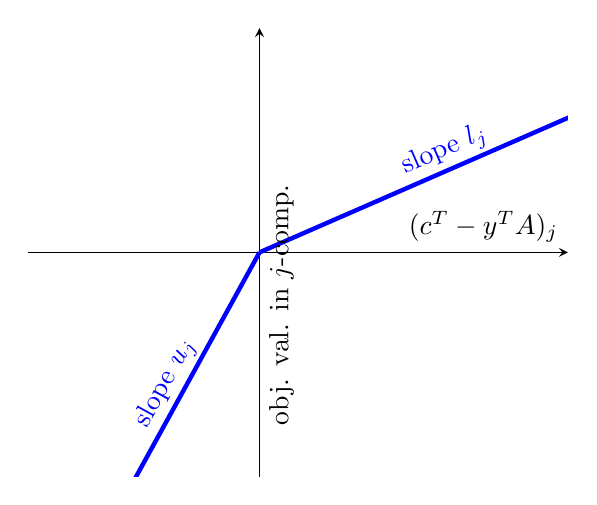
\begin{tikzpicture}
        \begin{axis}[
                axis x line=center,
                axis y line=middle,
                xlabel=$(c^T-y^TA)_j$,
                ylabel=obj. val. in $j$-comp.,
                ylabel style={sloped, xshift=-100pt},
                xmin=-3,
                xmax=4,
                ymin=-4,
                ymax=4,
                grid=none,
                ticks=none,
                % minor tick num=1,
                % axis equal image,
            ]
            \addplot[blue, ultra thick] coordinates {(0,0) (5,3)}
            node[pos=0.5, yshift=7pt,sloped]{slope $l_j$}
            ;
            \addplot[blue, ultra thick] coordinates {(-2,-5) (0,0)}
            node[pos=0.5, yshift=7pt,sloped]{slope $u_j$}
            ;
        \end{axis}
    \end{tikzpicture}
\end{minipage}
As can be seen in the plot, the cost function is concave!
